\documentclass[10pt]{article}

\usepackage{spheric}
%%%TITLE
\title{Corrected smoothed particle hydrodynamics for simulating
failure progress of model-scale ice}
\date{}

%%AFFILIATIONS

\author[1]{Xing ZHENG$^\dagger$}
\author[1]{Ningbo ZHANG}
\author[2]{Qingwei MA}

\affil[1]{Harbin Engineering University, China}
\affil[2]{City University London, UK}
\affil[$\relax$]{\email{\dagger}{zhengxing@hrbeu.edu.cn}}


%%DOCUMENT
\begin{document}

\maketitle

%\SelectedTopics{}

%%PLEASE PUT YOUR ABSTRACT HERE
\begin{abstract}
A corrected SPH method based on simplified finite difference interpolation method (SPH\_SFDI) is presented to simulate the failure process of ice. The Drucker-Prager model is applied into the SPH code to simulate four point bending and uniaxial compression failure of sea ice in model scale. To validate the SPH\_SFDI method, the numerical results of SPH\_SFDI are compared with SPH and experimental results. The good agreement with experimental data has demonstrated that the presented SPH\_SFDI procedure can be a useful numerical tool for the simulation of failure progress of ice.

SPH\_SFDI model which including the use of the elasto-plastic cohesion softening model is presented to simulate the bending and compression failure process of mode-scale ice. The predicted force in four-point bending and axial stress of the uniaxial compressive test are in good agreement with the experimental results. The predictions of fracture pattern are reasonable and acceptable. The conducted studies confirmed that the SPH\_SFDI method can be effectively used simulate physical destruction phenomena which occur during the failure process of ice. According to the comparisons between the numerical results conducted by SPH and SPH\_SFDI methods, and the experimental data, the performance of SPH\_SFDI is found better satisfactory than that of original SPH in view of accuracy and stability for simulating the bending and compression failure process of mode-scale ice.

\begin{figure}[!htb]
\centering
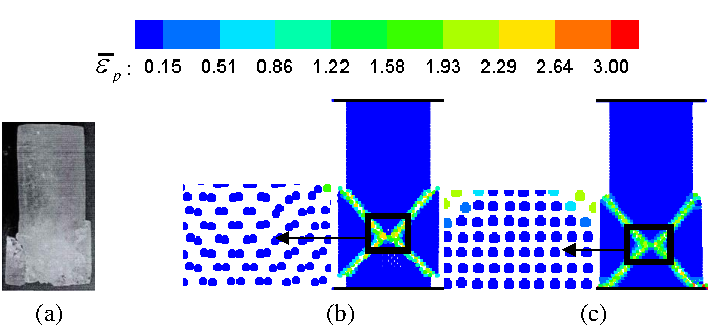
\includegraphics[width=0.85\textwidth]{41-1.pdf}
\caption{Comparison of the SPH (b) and SPH\_SFDI (c) simulation (contours of accumulated plastic strain) with a typical experimental bulge fracture pattern (a).}\label{fig:41}
\end{figure}

\end{abstract}


%%THE END OF ABSTRACT

\addbib

\end{document}
